\documentclass{acm_proc_article-sp}
\usepackage{balance}
\usepackage{algorithmic}
\usepackage{algorithm}
\usepackage{graphicx}
\usepackage{tabularx}
\usepackage{subfigure}


\begin{document}

\title{Breeding swarm: a hybrid PSO and GA}
\subtitle{Swarm Intelligence, natcomp.liacs.nl}
\numberofauthors{1}
\author{
\alignauthor
Xiwen Cheng\\
       \affaddr{Leiden Institute of Advanced Computer Science}\\
       \affaddr{Niels Bohrweg 1}\\
       \affaddr{Leiden, The Netherlands}\\
       \email{xcheng@liacs.nl}
}
\date{\today}

\maketitle
\begin{abstract}
In this essay Breeding Swarm, a hybrid of Particle Swarm Optimzer and Genetic Algorithm is analyzed by benchmarking it on the Ackley, Griewank and Rastrigrin functions. The reasoning behind combining these two types of optimizers is that PSO is best in exploitation while GA ensures diversity in the population, thus exploration. The main objective is to confirm the effectiveness of combining the two optimizers and what their contributions are to the hybrid algorithm. 
\end{abstract}

\section{Introduction}
Breeding Swarm (BS) is a hybrid variant introduced by Settles and Soule~\cite{SET05}. This hybrid combines Particle Swarm Optimizer (PSO) with Genetic Algorithm (GA). They showed it performs as good as their singular counterparts or sometimes even better by comparing the three in training an Artificial Recurrent Neural Network~\cite{SET052}.

In this document the effectiveness of BS is tested on four standard test functions. Namely the famous generalized Ackley function~\cite{ACK87, BAC96}, Griewank\cite{LOC03}, Rastrigin~\cite{MUH91} and Rosenbrock~\cite{MUL73}. In short the algorithm described in the original paper by Settles and Soule was implemented and tested against the benchmark optimization functions. To verify the hybrid does indeed yield better results, the subsystems \emph{PSO} and \emph{GA} were tested individually where possible. The GA part was improved by introducing \emph{uniform crossover} along with \emph{VPAC} (Velocity Propelled Averaged Crossover) proposed by Settles and Soule.

In sections~\ref{sec:pso},~\ref{sec:ga} and~\ref{sec:bs} the algorithms are outlined. Section \ref{sec:test} lists the test functions used to benchmark the algorithms. Followed by section~\ref{sec:params} and~\ref{sec:results} describing the used parameters and results respectively. Finally this document is ended with conclusions in section~\ref{sec:conclusions}.

\section{Particle Swarm Optimizer}\label{sec:pso}
Particle Swarm Optimizer is inspired by the behavour of bird flocking. It was proposed by Kennedy and Eberhart~\cite{KEN95} in 1995. A population, called \emph{swarm} having candidate solutions (\emph{particles}) represents a state of the algorithm. The position of a particle is updated based on its memory influenced by best solutions found so far. It is best described in an algorithm in the next section.

\subsection{Standard PSO}
It begins with randomly initializing the positions and velocities of each particle in the swarm, being in time $t = 0$. The fitness of each particle in the swarm is evaluated. A personal best $pBest$ and a neighbour best $nBest$ are selected. In some cases $nBest$ is called $gBest$ when the algorithm accounts all particles as being neighbours. For a number of iterations, or until an objective criteria is met do the following:
Update the velocity of each particle using the equation described in section~\ref{ssec:velocity}. Use the newly calculated velocity to update the particle's location. Evaluate the fitness of the new position, update $pBest$ and $nBest$ if necessary. See algorithm~\ref{algo:pso} for the algorithm outline.

  \begin{algorithm}[h]
  \begin{algorithmic}
    \STATE $t \gets 0;$
    \STATE $randomly\: initialize\: V(t);$
    \STATE $randomly\: initialize\: P(t);$
    \STATE $evaluate\: P(t);$
    \STATE $update\: pBest;$
    \STATE $update\: nBest;$
    \REPEAT
      \STATE $V(t+1) \gets updateVelocity(V(t));$
      \STATE $P(t+1) \gets P(t) + V(t+1);$
      \STATE $evaluate\: P(t+1);$
      \STATE $update\: pBest;$
      \STATE $update\: nBest$
      \STATE $t \gets t + 1;$
    \UNTIL{$stop\: requirement$}
  \end{algorithmic}
  \caption{Standard PSO algorithm}\label{algo:pso}
  \end{algorithm}

\subsection{Velocity and Position update}\label{ssec:velocity}
The new velocity denotes the direction and speed driving a particle. This is updated based on several social factors: $pBest$, $nBest$, etc... Formally the velocity and position are updated as follow:\\
\\
  \begin{eqnarray*}
   V(t+1) &=  & w \times V(t) \\
          &   & + c_{1} \times rand_{1}() \times (pBest - P(t)) \\
          &   & + c_{2} \times rand_{2}()\times (nBest - P(t)) \\
   P(t+1) &=  & P(t) + V(t+1)
  \end{eqnarray*}
\\
\\
Where:\\
  \begin{tabular}{lll}
    $pBest$           & =  & best solution found so far by the particle \\
    $nBest$           & =  & best solution found by $n$ neighbourhood \\
    $w$               & =  & inertia weight (damping weight) \\
    $c_1$, $c_2$      & =  & social parameters: memory and social \\
 &  & respectively \\
    $rand_1$, $rand_2$ & = & normal distributed random values \\
  \end{tabular}\\
\\
The maximum velocity is enforced using $vMax$. The social parameters dictate how strong the influences of $pBest$ and $nBest$ are. $w$ \emph{scales} the current velocity.

\section{Genetic Algorithm}\label{sec:ga}
Genetic Algorithm is inspired by evolution. Originally proposed by Holland in 1970's. In GA a population of bitstrings are used. Where a bitstring encodes candidate solutions. An individual is changed by crossover and mutation. The new population is composed of the newly created offspring. 

\subsection{Standard GA}
The population is also initialized randomly and then evaluated. For each consecutive generation mates are selected; they undergo crossover creating a set of offspring. The offspring are then mutated introducing new variants in the population. The offspring become the new population of which their fitnesses are evaluated. See algorithm ~\ref{algo:ga} for the formal outline.
\begin{algorithm}[h]
  \begin{algorithmic}
    \STATE $t \gets 0;$
    \STATE $initialize\: P(t);$
    \STATE $evaluate\: P(t);$
    \REPEAT
      \STATE $P'(t) \gets select\mbox{-}mates(P(t));$
      \STATE $P''(t) \gets crossover(P'(t), p_c);$
      \STATE $P'''(t) \gets mutation(P''(t), p_m);$
      \STATE $evaluate\: P'''(t);$
      \STATE $P(t+1) \gets P'''(t);$
      \STATE $t \gets t + 1;$
    \UNTIL{$stop\: requirement$}
  \end{algorithmic}
\caption{Standard GA}\label{algo:ga}
\end{algorithm}
\subsection{Operators}
GA has several types of operators. They are \emph{selection}, \emph{crossover} and \emph{mutation}. In turn each type can be implemented in different ways exhibiting different behaviors. 

\subsubsection{Selection}
This operator selects which individual is allowed to mate. The most general forms are proportional where the probability of a individual being selected is proportional to its fitness with regard to the total fitness of the population. Another variant is tournament selection where two individuals compete with each other, the winner (better fitness) is selected.
\subsubsection{Crossover}
Two parents are randomly selected from the candidate mates and recombined into two offspring. The general types of recombination are single point, two point and uniform. In single point, one point in the bitstring is randomly chosen, cut and swap the substrings. For two points it happens in the same way, but with two crossover points. In uniform each bit is swapped with a probability, mostly $p_c = 0.5$.
\subsubsection{Mutation}
In mutation each bit in the bitstring is flipped with a probability $p_m$. This operator guarantees variety in the population and therefore increases explorative ability. A crucial property in finding the global optimum and not getting stuck at a local optimum.

\section{Breeding Swarm}\label{sec:bs}
It is important to note that the effectiveness of PSO greatly depends on the initial population. Because particles are driven by their social knowledge, it may never find the global optimum. However, if it searches at the \emph{correct} area (being near the global optimum) it will be able to find better solutions. On the other side GA's are not that great at fine tuning solutions but thrives in being explorative. See table~\ref{tbl:compare} for the comparison between these two. Breeding swarm (BS) combines the ideas of using velocity and position update rules of PSO with the selection, crossover and mutation mechanism of GA.
\begin{table}[h]
    \begin{tabularx}{0.47\textwidth}{|X|X|}
    \hline
    \textbf{PSO} & \textbf{GA} \\
    \hline
    Directional updates & Omnidirectional mutation\\
    Mixes neighbours & Mixes \emph{random} individuals\\
    Exploitative & Explorative\\
    \hline
    \end{tabularx}
    \caption{Comparison PSO and GA}\label{tbl:compare}
\end{table}

\subsection{Generic Hybrid Algorithm}
Just like other population based optimizers the initial population is randomly initialized. Because PSO is part of the algorithm each particle has its own velocity, hence they are also initialized in the same fashion. The initial population is then evaluated. In the evolution loop a subset of best candidates are selected. A copy of this subset, $P_{pso}$ undergoes velocity and location update as described in PSO. The rest is constructed using GA with crossover and mutation. See algorithm~\ref{algo:hb}.

\begin{algorithm}[h]
  \begin{algorithmic}
    \STATE $t \gets 0;$
    \STATE $initialize\: P(t), V(t);$
    \STATE $evaluate\: P(t);$
    \REPEAT
      \STATE $P_{elite}(t) \gets copyBest(P(t), N_{elite});$
      \STATE $P_{pso}(t) \gets select_1(P_{elite}(t), (N - N_{elite}) * \Psi);$
      \STATE $V'(t) \gets updateVelocity(V(t), P_{pso}(t));$
      \STATE $P'_{pso}(t) \gets updatePosition(P_{pso}(t), V'_{pso}(t));$
      
      \STATE $P_{ga}(t) \gets select_2(P_{elite}(t), (N - N_{elite}) * (1-\Psi));$
      \STATE $P'_{ga}(t) \gets crossover(P_{ga}(t), p_c);$
      \STATE $P''_{ga}(t) \gets mutation(P'_{ga}(t), p_m);$
      
      \STATE $P(t+1) \gets P_{elite} \cup P'_{pso} \cup P''_{ga};$
      \STATE $V(t+1) \gets V'(t);$
      \STATE $evaluate\: P(t+1);$
      \STATE $t \gets t + 1;$
    \UNTIL{$stop\: requirement$}
  \end{algorithmic}
  \caption{Generic Hybrid algorithm}\label{algo:hb}
\end{algorithm}
Where:\\
  \begin{tabular}{ll}
  $ N $ & Number of individuals \\
  $ N_{elite} $ & Number of elites \\
  $ \Psi $ & \emph{Breeding ratio}, proportion that undergoes \\
  & breeding; [0.0:1.0]\\
  $ select_1, select_2 $ & Two selection methods, may be different\\
  $ p_c, p_m $ & Crossover rate and mutation rate \\
  & respectively \\
  \end{tabular}
\subsection{Breeding Swarm Algorithm}
Breeding Swarm is an instantiation of the hybrid algorithm described above. It uses tournament selection and a non-standard crossover operator named VPAC(See section \ref{ssec:vpac}. The mutation operator mutates each individual with probability $p_m$. See figure~\ref{fig:bs} for the evolution loop. It is designed such that GA performs global search and PSO performs local search.
Standard velocity and position update rules are used. However: \\
  \begin{tabular}{ll}
  $N_{elite}$ & $ = 0$\\
  $\Psi$ & $ = 0.5, $ even distribution between PSO \\
  & and GA \\
  $select_1 = select_2 $ & $ = $ tournament selection with size of 2\\
  $crossover$ & $ = $ \emph{VPAC} \\
  $mutation$ & $ = $ Gaussian with mean 0 and variance \\
  & reduced linearly each generation from \\
  & 1.0 to 0.0 \\
  $inertia \: weight$  & $ = $ reduced linearly each generation \\
  & from 0.7 to 0.4 \\
  $social \: parameter$ & $ = 2$, $c1 \mbox{ and } c2$ in position update\\
  $V_{max} $ & $ = \pm 1$ \\
  \end{tabular}

\begin{figure}[h]
\centering
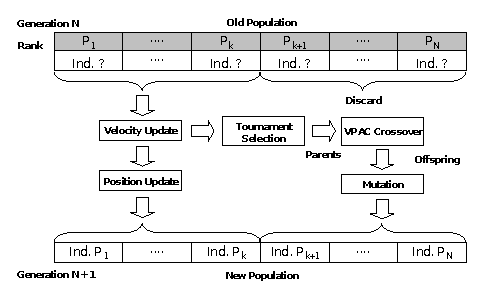
\includegraphics[scale=1.0]{figbs.eps}
\caption{Breeding Swarm~\cite{SET052}}\label{fig:bs}
\end{figure}

\subsection{Velocity Propelled Averaged Crossover}\label{ssec:vpac}
Because GA operators normally operate on bitstrings, a special crossover was developed that uses velocity. VPAC proposed by Settles and Soule takes the overage velocity of two individuals and then update the location according to the following rule:
  \begin{equation}
   c_1(x_i) = \frac{p_1(x_i) + p_2(x_i)}{2.0} - \varphi_1 p_2(v_i)
  \end{equation}
  \begin{equation}
   c_2(x_i) = \frac{p_1(x_i) + p_2(x_i)}{2.0} - \varphi_2 p_1(v_i)
  \end{equation}
  \bigskip
  Where:\\
  \bigskip
  \begin{tabular}{ll}
  $c_1(x_i), c_2(x_i) $ & Positions of childrens in dimension $i$\\
  $p_1(x_i), p_2(x_i) $ & Positions of parents in dimension $i$\\
  $p_1(v_i), p_2(v_i) $ & Velocities of parents in dimension $i$\\
  $\varphi_1, \varphi_2 $ & Uniform random variable in [0.0:1.0]\\
  \end{tabular}\\
The idea is to accelerate away from parent's current direction and therefore increase diversity in the population.

\section{Implemented optimizers}\label{sec:optimizers}
To compare the BS proposed by Settles and Soule, some simplified variants of BS were implemented. This is needed to analyze how the each segment of the algorithm performs individually. The algorithms were implemented in a single matlab function:
\begin{eqnarray*}
 [fxmin, xmin, history] = & bs(objfunc, args, dim, n, \\
    & s, i, vmax, xmax, mode)
\end{eqnarray*}

Where:\\
\begin{tabular}{lll}
$objfunc$   & = & name of objective function to be \\
           &   & minimized\\
$args$      & = & set of constant arguments passed \\
            & & to $objfunc$\\
$dim$       & = & dimension of an individual\\
$n$         & = & population size\\
$s$         & = & survivors, where:\\
          & $s == 0$ & -> GA with VPAC\\
          & $s == n$ & -> plain PSO\\
          & $0 < s < n$ & -> BS\\
$i$         & = & number of iterations to run\\
$vmax$      & = & maximum velocity\\
$xmax$      & = & maximum x\\
$mode$      & = & Crossover mode, where:\\
      & $mode == 0$ & -> VPAC only\\
      & $mode == 1$ & -> uniform crossover only\\
      & $mode == 2$ & -> VPAC then uniform crossover\\
      & $otherwise$ & -> no crossover at all\\
\end{tabular}\\
And the return values:\\
\begin{tabular}{lll}
$fxmin$ & = & best fitness \\
$xmin$ & = & best individual corresponding to $fxmin$\\
$history$ & = & best solution per iteration\\
\end{tabular}\\

The behaviour of the algorithm can be influenced using the $s$ variable and by setting a $mode$. Whenever $s = n$, BS behaves like a normal PSO because no particles undergo breeding. And for $s = 0$ the algorithm assumes no particle is updated by PSO and thus is the equivalence of performing GA operations only. In this case the velocities remain unchanged between generations!
$mode$ changes what type of crossover is applied. In uniform crossover, elements of two parents are swapped with probability $p_c = 0.5$ to create new offspring.
In total 7 combinations were tested:\\

\begin{tabularx}{0.3\textwidth}{lll}
GA0 & = & no PSO, VPAC only\\
GA1 & = & no PSO, Uniform Crossover only\\
GA2 & = & no PSO, VPAC then Uniform Crossover\\
PSO & = & no GA\\
BS0 & = & PSO, GA with VPAC only\\
BS1 & = & PSO, GA with Uniform Crossover only\\
BS2 & = & PSO, GA with VPAC then Uniform Crossover\\
\end{tabularx}

\section{Test functions}\label{sec:test}
In order to analyze the behaviours of the algorithms they were put to the test against four well known test functions. In contrast to the original paper, this hasn't been done. 

\subsection{Ackley}
The Ackley~\cite{ACK87} problem is a minimzation problem. It has been generalized to $N$ dimensions~\cite{BAC96}:

\begin{eqnarray*}
    \mathop{F(\vec{x})}&=&-20\cdot exp(-0.2\sqrt{\frac{1}{n}\cdot\sum\limits_{i=1}^{n}x_{i}^{2}})\\
                    &&- exp(\frac{1}{n}\cdot\sum\limits_{i=1}^{n}\cos(2\pi
                    x_{i})) + 20 + exp(1)
\end{eqnarray*}
Figure~\ref{fig:ackley} shows a plot of the Ackley function in two dimensions.  We can observe that it has a large quantity of local optimas with a single global optimum $\vec{x} = (0_1, ..., 0_n)$ with $F(\vec{x}) = 0$.
\begin{figure}[ht]
\centering
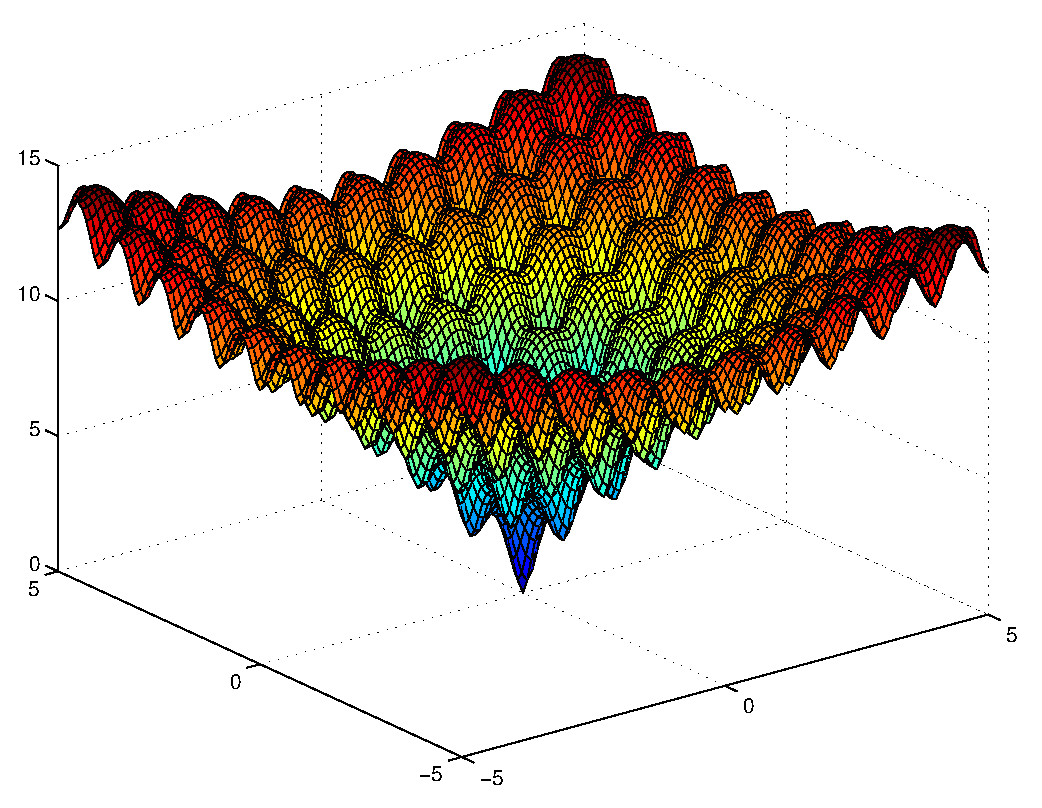
\includegraphics[scale=0.4]{fig-ackley}
\caption{Ackley function in two dimensions}\label{fig:ackley}
\end{figure}

\subsection{Griewank}
The Griewank test function is also interesting to look at because it has an enormous amount of local minimas with a single optima $\vec{x} = (0_1, ..., 0_n)$, just like the Ackley function:
\begin{eqnarray*}
\mathop{F(\vec{x})} &=& \sum\limits_{i=1}^{n}\frac{x_i^2}{4000} - \prod\limits_{i=1}^{n}\frac{cos(x_i)}{\sqrt{i}} + 1
\end{eqnarray*}

Note that the distance between optimas are larger compared to the Ackley function given the same search space size. Figure~\ref{fig:griewank} is plotted on the same scale as the rest. 
\begin{figure}[ht]
\centering
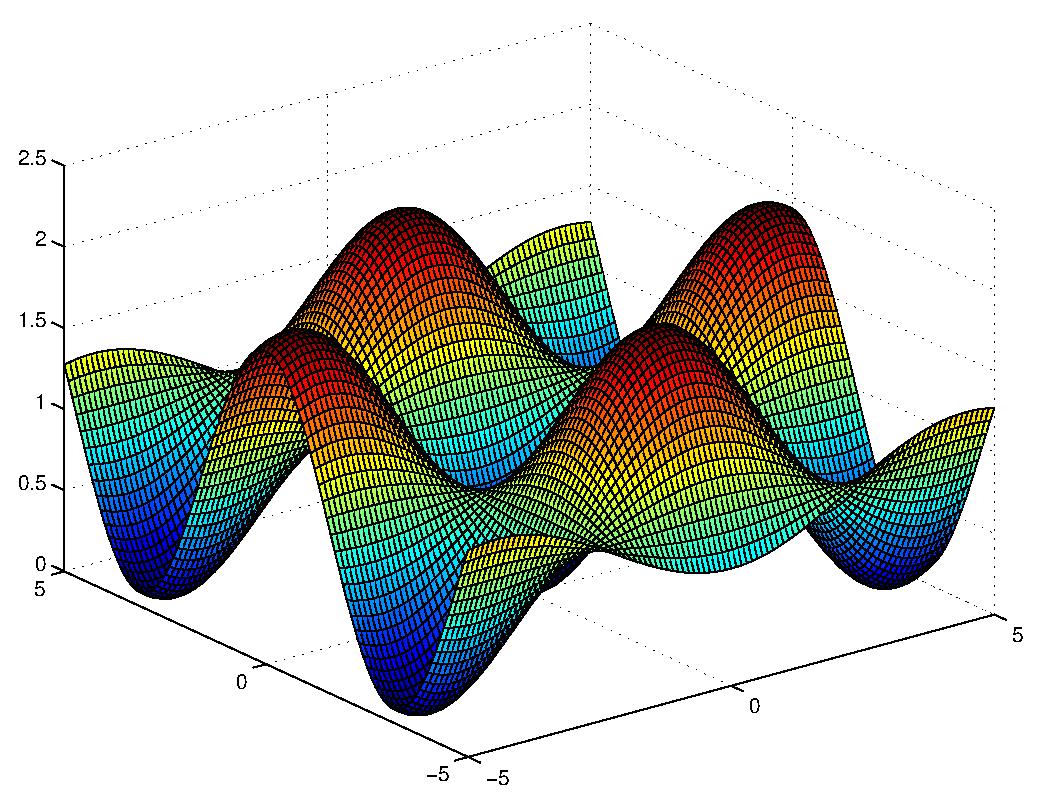
\includegraphics[scale=0.4]{fig-griewank}
\caption{Griewank function in two dimensions}\label{fig:griewank}
\end{figure}

\subsection{Rastringrin}
The Rastrigrin function is also similar to the previous two. However given the same search space size it contains way more local optimas. So this is very \emph{dense} (See figure~\ref{fig:rastrigrin}). Its corresponding equation is as follow:
\begin{eqnarray*}
\mathop{F(\vec{x})} &=& n \cdot 10 + \sum\limits_{i=1}^{n})[x_i^2 - 10 \cdot cos(2\pi x_i)]
\end{eqnarray*}

\begin{figure}[ht]
\centering
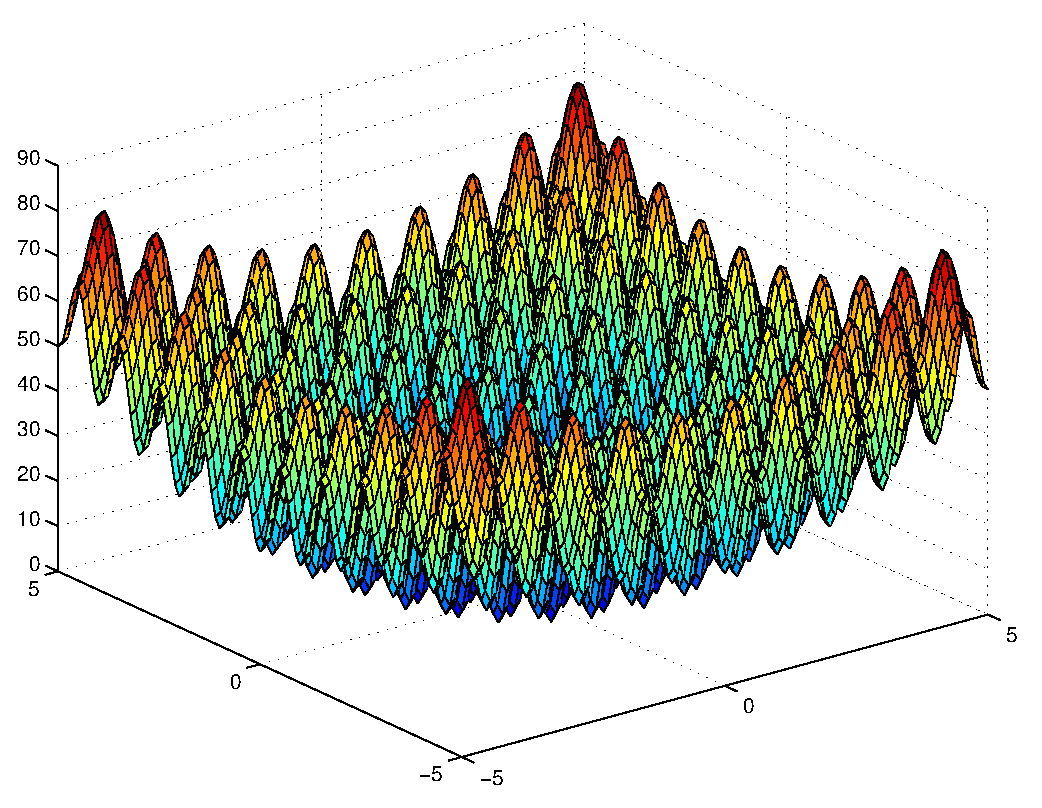
\includegraphics[scale=0.4]{fig-rastrigrin}
\caption{Rastrigrin function in two dimensions}\label{fig:rastrigrin}
\end{figure}

\subsection{Rosenbrock}
Rosenbrock is the simplest in terms of number of optimas (See figure~\ref{fig:rosenbrock}). However they are not trivial to converge to them. The global optimum is the vector $\vec{x} = (1_1, ..., 1_n)$. The function looks as follow:
\begin{eqnarray*}
\mathop{F(\vec{x})} &=& \sum\limits_{i=1}^{n-1}[100 \cdot (x_{i+1} - x_i^2)^2 + (1-x_i)^2]
\end{eqnarray*}

\begin{figure}[ht]
\centering
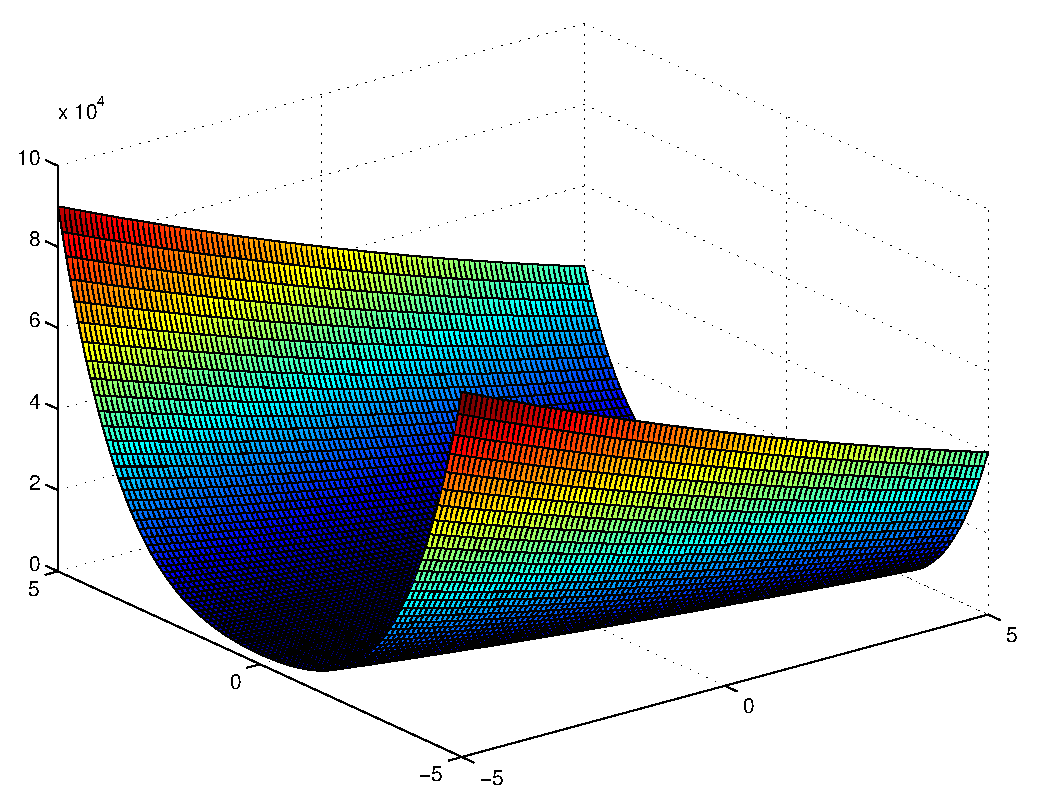
\includegraphics[scale=0.4]{fig-rosenbrock}
\caption{Rosenbrock function in two dimensions}\label{fig:rosenbrock}
\end{figure}

\section{Parameters}\label{sec:params}
Each function was tested using the algorithms listed in section~\ref{sec:optimizers}. Some parameters has been set statically while others changed linearly. These parameters are:\\

\begin{tabular}{lll}
$N$ & = & 40, population size\\
$s$ & = & 20, number of survivors\\
$d$ & = & 200, dimensionality\\
$i$ & = & 300, number of iterations\\
$inertia$ & = & decreases from 0.7 to 0.4 proportional\\
&& to $i$, inertia weight\\
$p_m$ & = & decreases from 1 to 0 proportional to $i$,\\
&& mutation rate\\
$p_c$ & = & 0.5, crossover rate\\
$vmax$ & = & 1, maximum velocity\\
$xmax$ & = & 10, maximum values\\
$runs$ & = & 20, number of runs per algorithm per \\
&& function\\
\end{tabular}

\section{Results}\label{sec:results}
For each test function there are two graphs. One containing the mean plots of each algorith. The other on the right is its corresponding standard deviations. It is remarkable that \emph{BS1} performs best in 4 out of 4 functions (figures~\ref{gra:ackley}-\ref{gra:rosenbrock} when it comes to finding good solutions. The Rosenbrock results (figure~\ref{gra:rosenbrock}) is very interesting because almost all algorithms converge at the same pace except \emph{PSO}.

Plain \emph{PSO} performs the worse in all cases. This is mainly the case because of the many \emph{traps} it could fall into which it fails to explore the search space for potential better solutions. However the standard deviation of 3 out of 4 (figures~\ref{gra:griewank}-\ref{gra:rosenbrock}) is fairly high compared to the others. This gives the impression it doesn't exploit its social behavior that well. The reason is probably that it jumps between local optimas of the similar fitnesses. This could be helped by reducing the maximum velocity over time.

The overall convergence speed is highest in all cases at the very beginning. The algorithms begin to stagnate very quickly right after. This is probably the result of $p_m$ and $inertia$ being too low to introduce actual change in the population. This raises the question whether linearly decreasing those parameters is a good idea. Perhaps a logaithmic reduction is more suitable to encourage exploration.

Back to the original question: Does combining PSO with GA really improve the performance? \emph{BS1} performs by far the best, but that's mainly because \emph{GA1} is already very good. Both uses \emph{Uniform Crossover} instead of \emph{VPAC}. For the Ackley and Griewank functions the other pair \emph{BS2} and \emph{GA2} shows slight increase of variane in the standard deviations. \emph{BS0}, proposed by Settles and Soule, decreases the variance compared to \emph{GA0}.

For the four test functions using uniform crossover yields better results then VPAC. Applying uniform crossover after VPAC doesn't seem to enhance the search strategy at all. The performance of Breeding Swarm greatly depends on the performance of the GA subsystem. The difference between a GA and its BS variant is quite small, but there's slight improvement.

\begin{figure*}[ht]
\centering
\mbox{\subfigure{
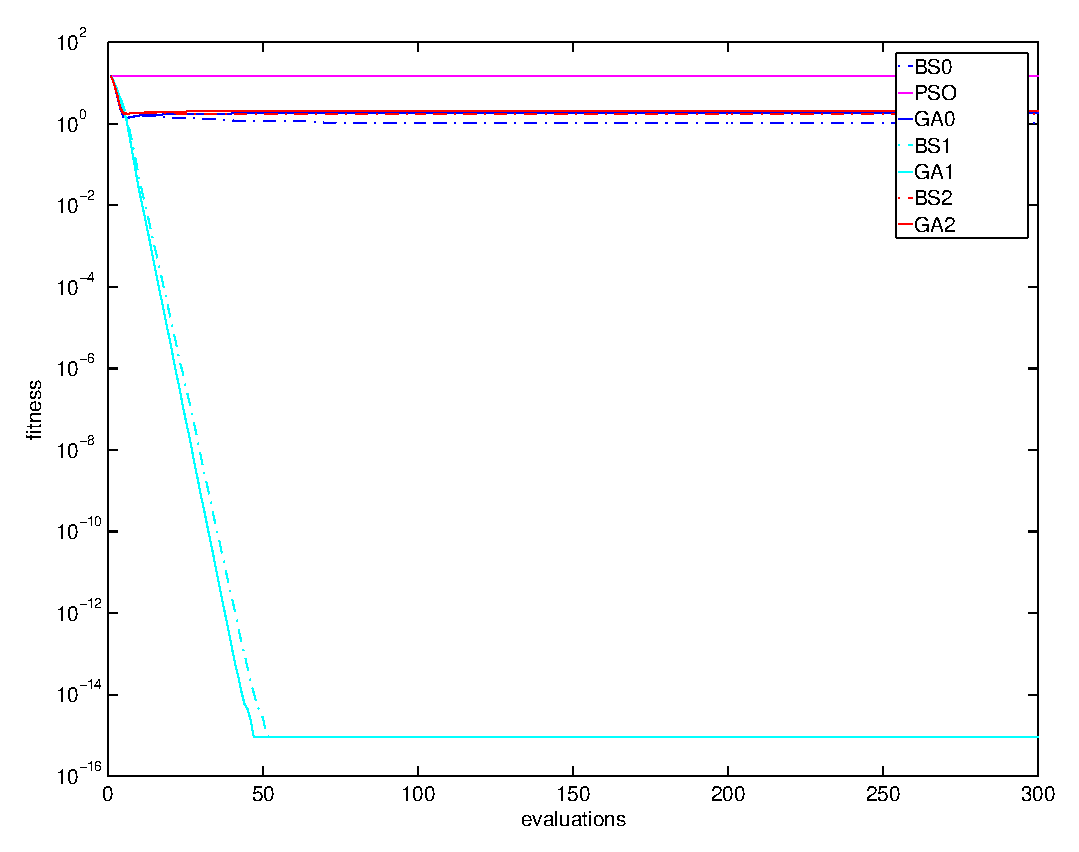
\includegraphics[scale=0.5]{output/obj_ackley-d200-s20-n40-all-mean}
}
\quad
\subfigure{
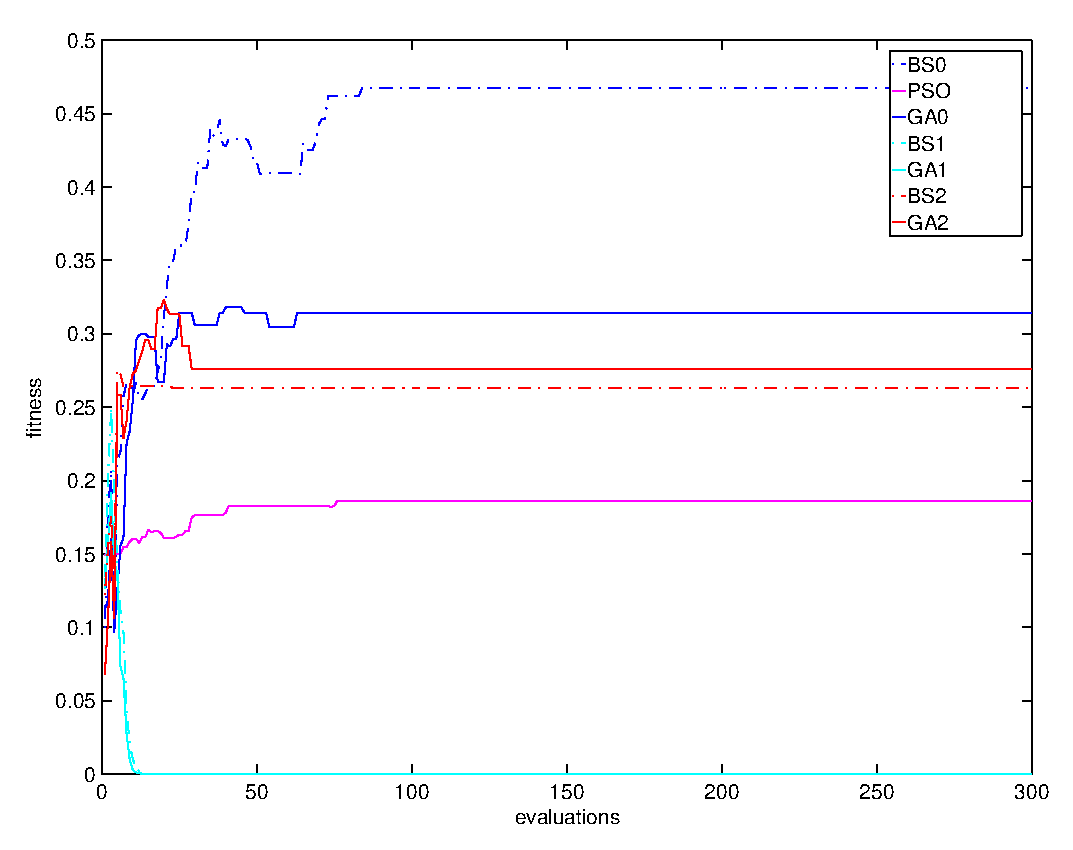
\includegraphics[scale=0.5]{output/obj_ackley-d200-s20-n40-all-std}
}
}
\caption{Ackley: mean and standard deviation}\label{gra:ackley}
\end{figure*}

\begin{figure*}[ht]
\centering
\mbox{\subfigure{
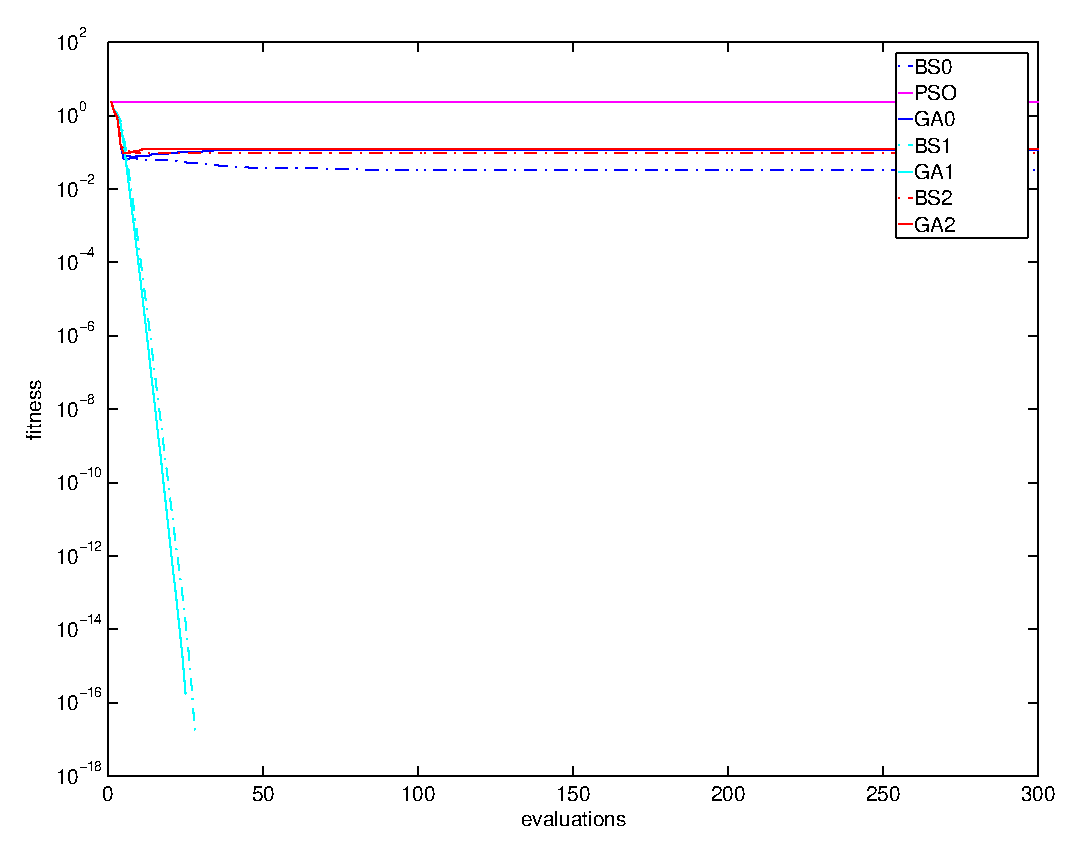
\includegraphics[scale=0.5]{output/obj_griewank-d200-s20-n40-all-mean}
}
\quad
\subfigure{
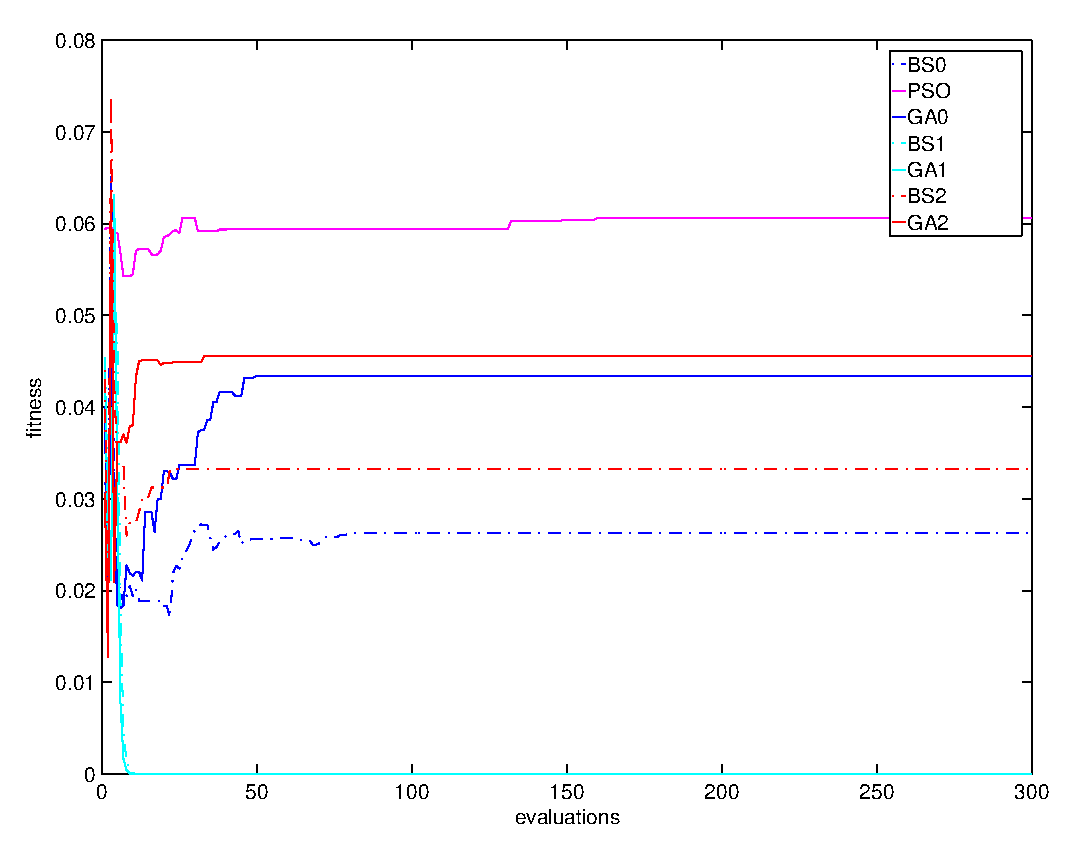
\includegraphics[scale=0.5]{output/obj_griewank-d200-s20-n40-all-std}
}
}
\caption{Griewank: mean and standard deviation}\label{gra:griewank}
\end{figure*}

\begin{figure*}[ht]
\centering
\mbox{\subfigure{
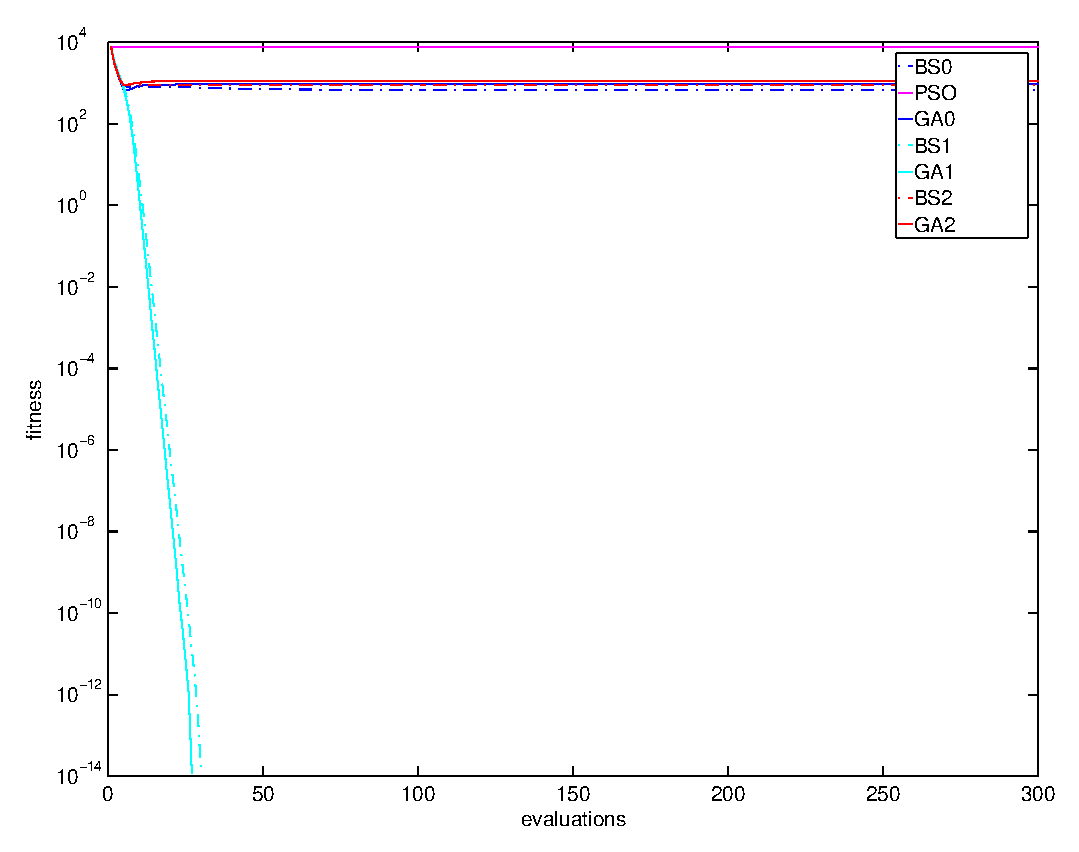
\includegraphics[scale=0.5]{output/obj_rastrigrin-d200-s20-n40-all-mean}
}
\quad
\subfigure{
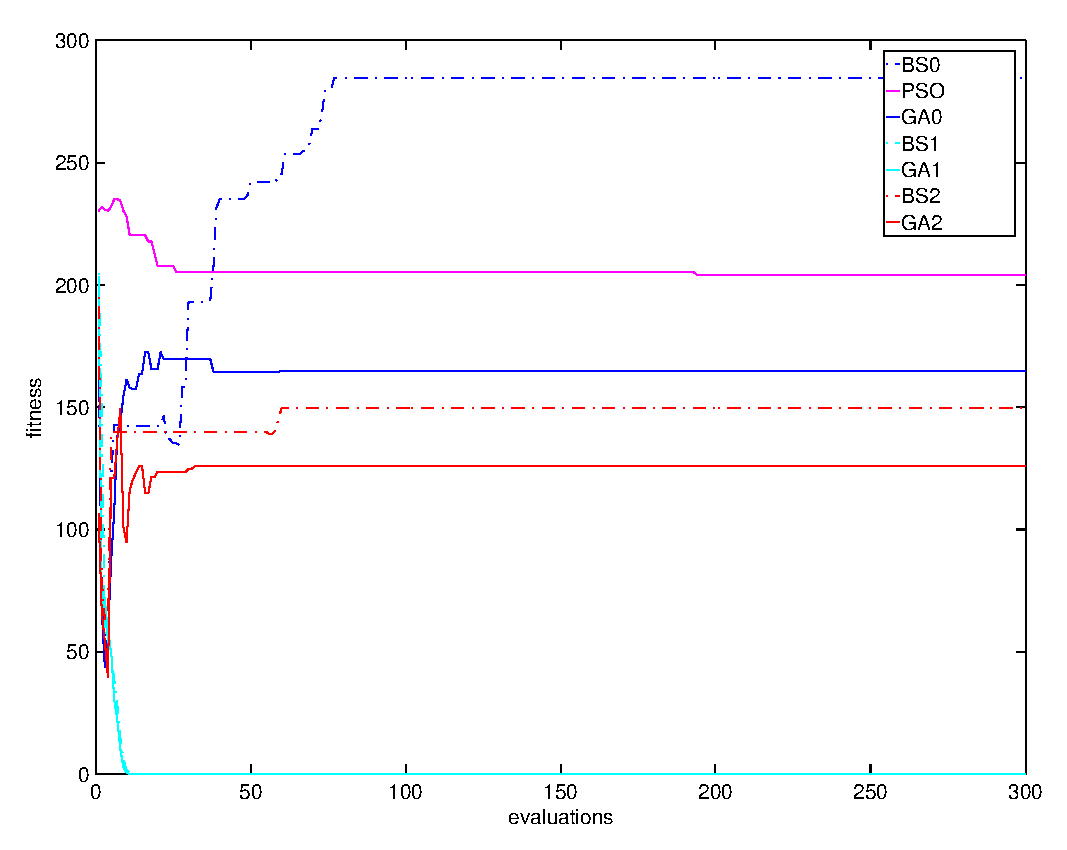
\includegraphics[scale=0.5]{output/obj_rastrigrin-d200-s20-n40-all-std}
}
}
\caption{Rastrigrin: mean and standard deviation}\label{gra:rastrigrin}
\end{figure*}

\begin{figure*}[ht]
\centering
\mbox{\subfigure{
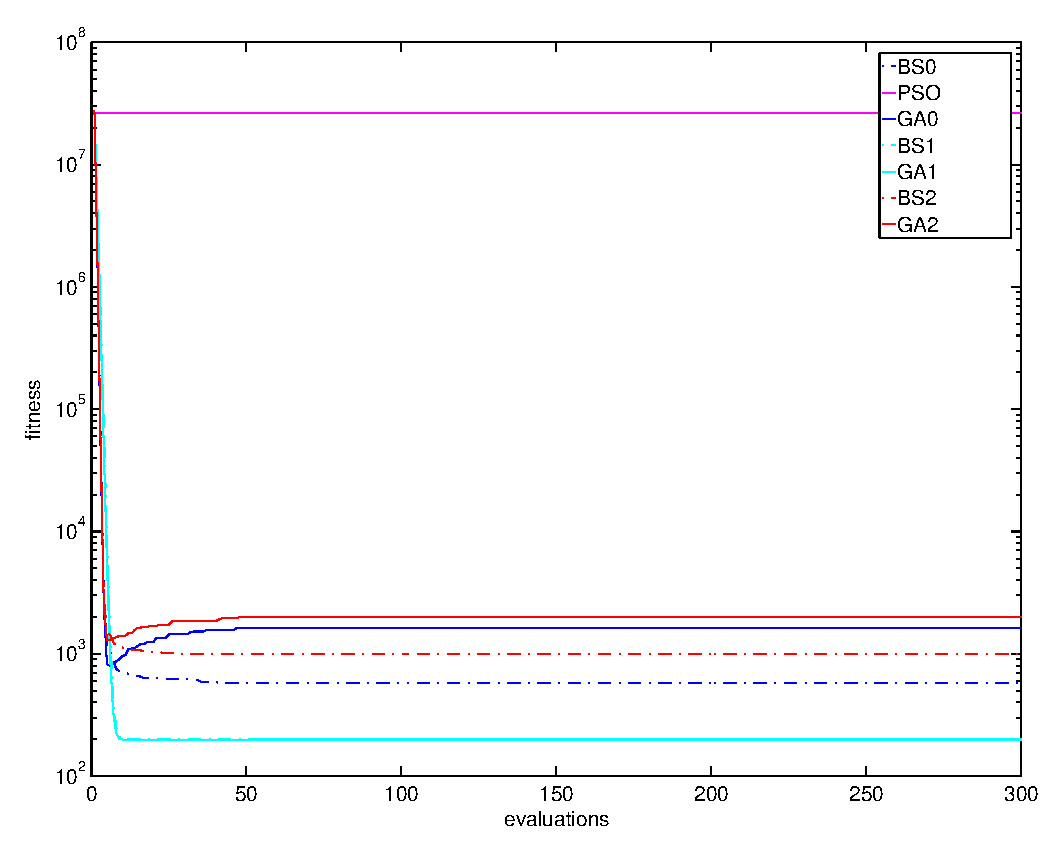
\includegraphics[scale=0.5]{output/obj_rosenbrock-d200-s20-n40-all-mean}
}
\quad
\subfigure{
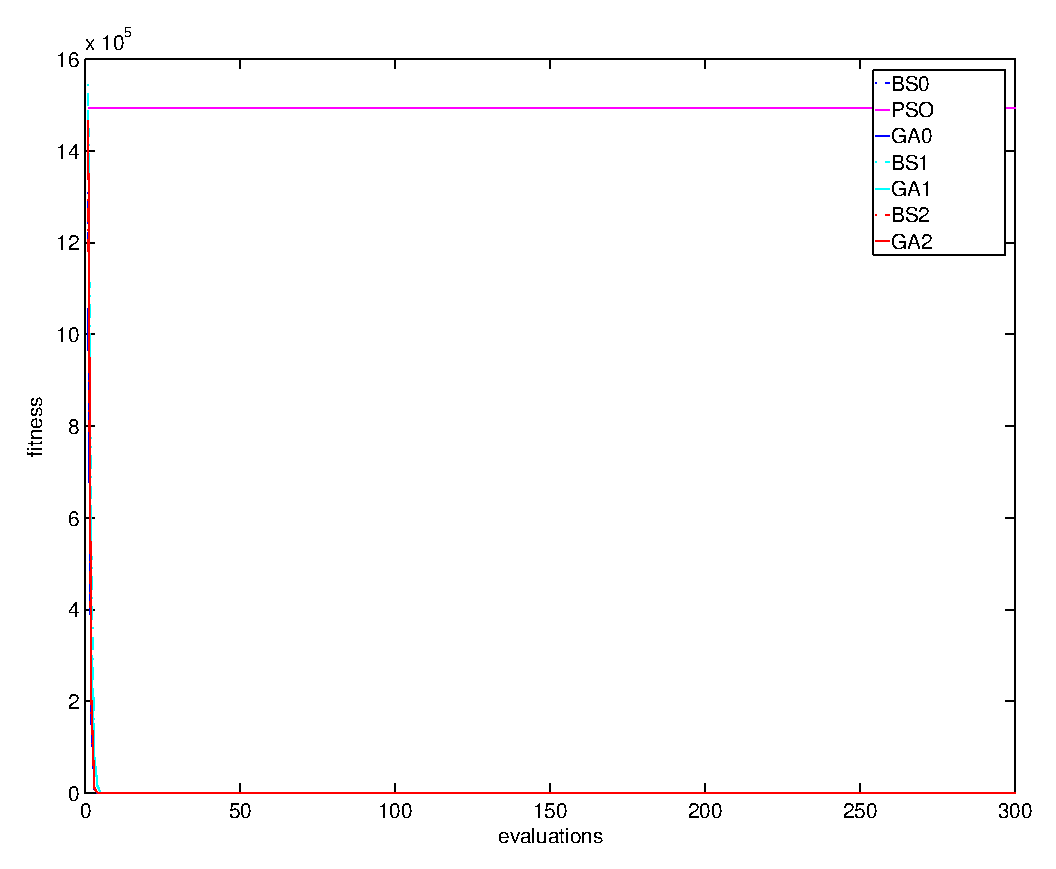
\includegraphics[scale=0.5]{output/obj_rosenbrock-d200-s20-n40-all-std}
}
}
\caption{Rosenbrock: mean and standard deviation}\label{gra:rosenbrock}
\end{figure*}

\section{Conclusions}\label{sec:conclusions}
In the results reported by Settles and Soule~\cite{SET052} the recurrent neural training exhibits a remarkable behavior: Quickest improvements occur towards the end of the run. However that is not the case in the results reported above. In fact the quickest improvements occur in the beginning of the runs. This is the biggest difference between the findings. As their actual algorithms weren't made public there's a high probability for the implementations to differ. 

Nevertheless their original idea is still valid: GA contributes for a great part in exploring the search space while PSO will fine-tune the solutions. Based on above results, it is probably better to distance from linearly decreasing the parameters and use a non-linear function with small slopes at the beginning like $ln(x)$. Or even better yet adopt self-adaptive idea from Evolutionary Strategies.

Combining these is not a bad idea at all. Eventhough PSO doesn't seem to contribute much to the algorithm. Where as it is clear from the results that BS relies heavily on the GA performance. PSO still is able to improve these results further. The margin may be small but noticable. 

Instead of mixing PSO and GA within one iterations, it is probably a good idea to \emph{chain} the optimizers. This is interesting when fitness evaluations are expensive. By using GA at the beginning the search space is explored for potential good candidates. Then PSO could optimize these candidates fine tuning the solutions. 

\bibliographystyle{abbrv}
\bibliography{sigproc}
\balancecolumns
\end{document}
